\section{Statecharts (nach Marwedel)}

\subsection{Nachteile von State-Event-Diagrammen}

\begin{itemize}
    \item Zustandsdiagramme sind flach (es gibt keine Hierarchie) \textrightarrow\ schnell unübersichtlicht
    \item Es kann keine zeitliche Parallelität modelliert werden
\end{itemize}


\subsection{Definitionen}

\begin{description}
    \item[active state:] Aktueller Zustand der FSM
    \item[basic states:] Zustände, die \textbf{nicht} aus anderen Zuständen bestehen
    \item[super states:] Zustände, die andere Zustände enthalten
    \item[ancestor states:] Für jeden basic state $s$ werden die super states, die $s$ enthalten, als \textbf{ancestor states} bezeichnet
    \item[OR-super-states:] Super-states $S$ werden OR-super-states genannt, wenn \textbf{genau einer} der sub-states von $S$ aktiv ist,
        wenn $S$ aktiv ist \textrightarrow\ Hierarchie
    \item[AND-super-states:] Super-states $S$ werden AND-super-states genannt, wenn \textbf{mehrere} der sub-states von $S$ \textbf{gleichzeitig} 
        aktiv sind, wenn $S$ aktiv ist \textrightarrow\ Parallelität \\
        \textrightarrow\ Werden auch \textbf{Teilautomaten} genannt
\end{description}

\begin{center}
    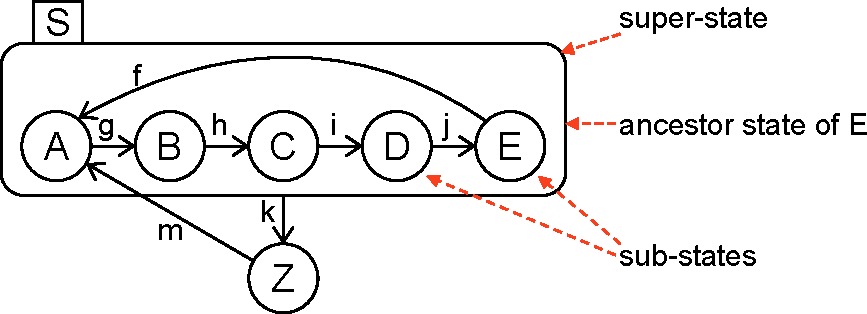
\includegraphics[width=0.85\columnwidth]{images/statechart_definition.pdf}
\end{center}


\subsubsection{Elemente der Statecharts}

\begin{center}
    % 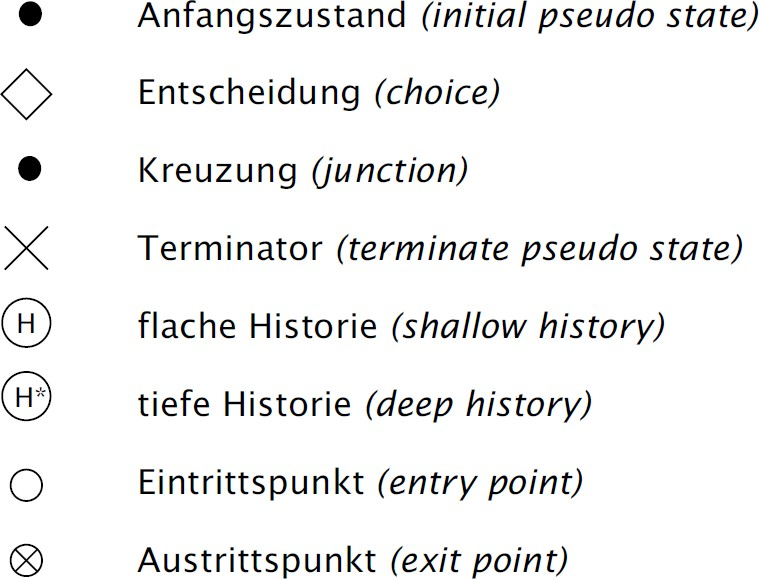
\includegraphics[width=0.7\columnwidth]{images/statechart_elements.jpeg}
    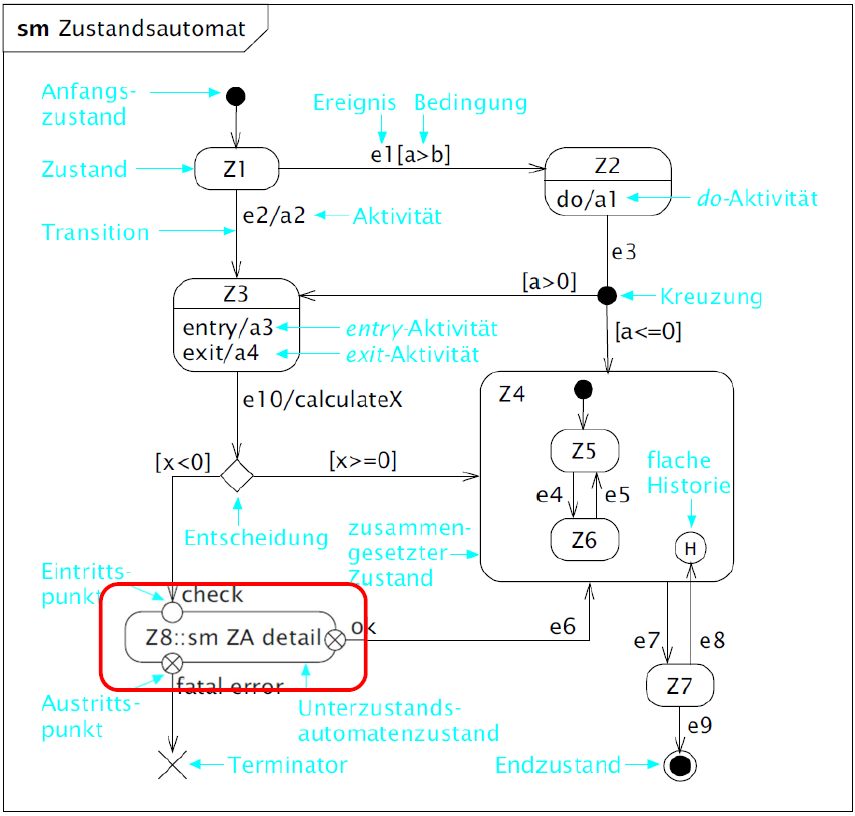
\includegraphics[width=0.7\columnwidth]{images/statechart_overview.png}
    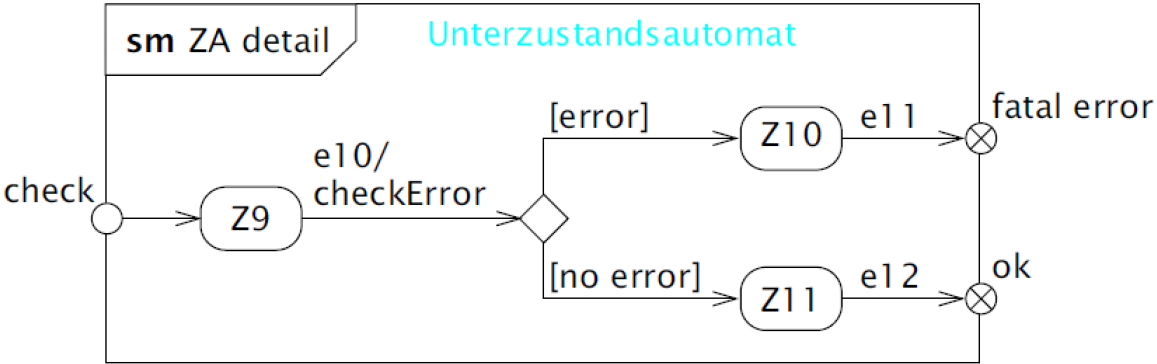
\includegraphics[width=0.6\columnwidth]{images/statechart_overview_submachine.png}
\end{center}


\subsubsection{Allgemeine Syntax für Transitions-Pfeile}

$$ \underrightarrow{\text{event [guard] / reaction}} $$

\begin{description}
    \item[event] auftretendes Event
    \item[guard] Bedingung, welche zutreffen \textbf{muss}, damit Zustand überhaupt gewechselt wird 
    \item[reaction] Zuweisung einer Variablen / Erzeugung eines Events beim Zustandswechsel 
\end{description}


\subsection{Hierarchie (OR-super-states)}

\begin{itemize}
    \item Die FSM befindet sich in \textbf{genau einem} sub-state von $S$, wenn $S$ aktiv ist.\\
        (\textrightarrow\ either in $A$ \textbf{OR} in $B$ \textbf{OR} ...)
\end{itemize}

\vspace{0.2cm}

\begin{minipage}[c]{0.41\columnwidth}
    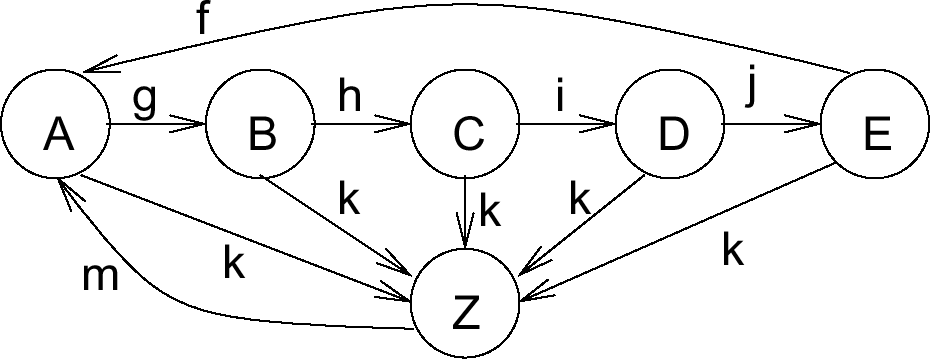
\includegraphics[width=\columnwidth]{images/statechart_unuebersichtlich.png}
\end{minipage}
\hfill
\begin{minipage}[c]{0.05\columnwidth}
    \begin{center}
        \huge \textrightarrow\
    \end{center}
\end{minipage}
\hfill
\begin{minipage}[c]{0.41\columnwidth}
    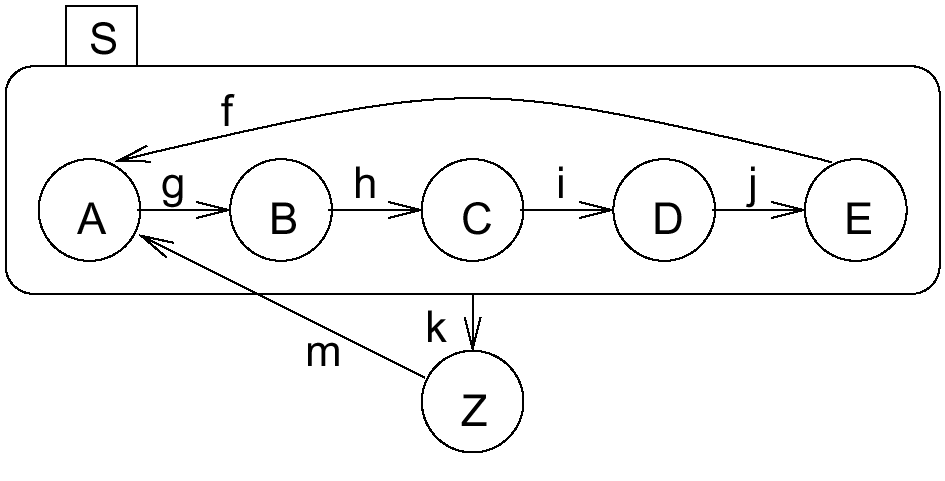
\includegraphics[width=\columnwidth]{images/statechart_hierarchie.png}
\end{minipage}


\subsection{Default-State}

\begin{itemize}
    \item Ziel: Interne Struktur des states vor der Aussenwelt verstecken \textrightarrow\ default state
    \item Ausgefüllter Kreis beschreibt den sub-state, welcher 'betreten' wird, wenn der super-state $S$ 'betreten' wird % CHECK: besseres Wort als betreten?
\end{itemize}

\vspace{0.2cm}

\begin{minipage}[c]{0.41\columnwidth}
    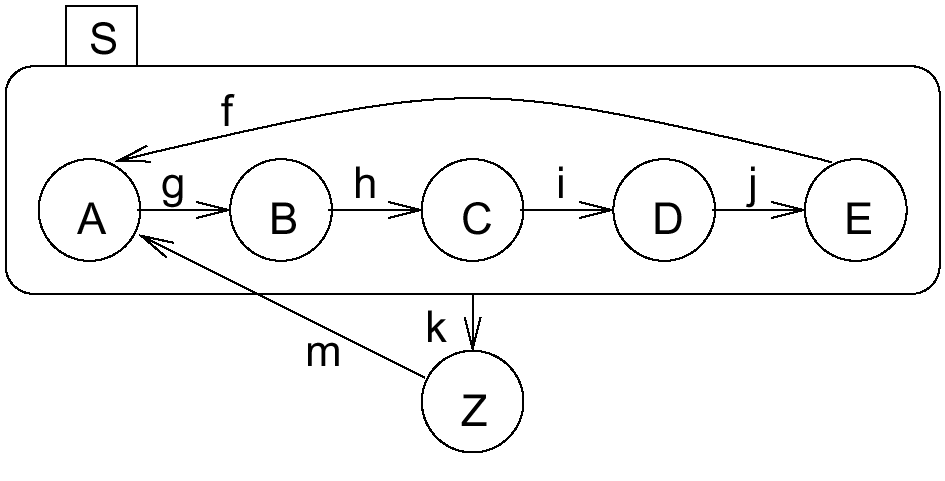
\includegraphics[width=\columnwidth]{images/statechart_hierarchie.png}
\end{minipage}
\hfill
\begin{minipage}[c]{0.05\columnwidth}
    \begin{center}
        \huge \textrightarrow\
    \end{center}
\end{minipage}
\hfill
\begin{minipage}[c]{0.41\columnwidth}
    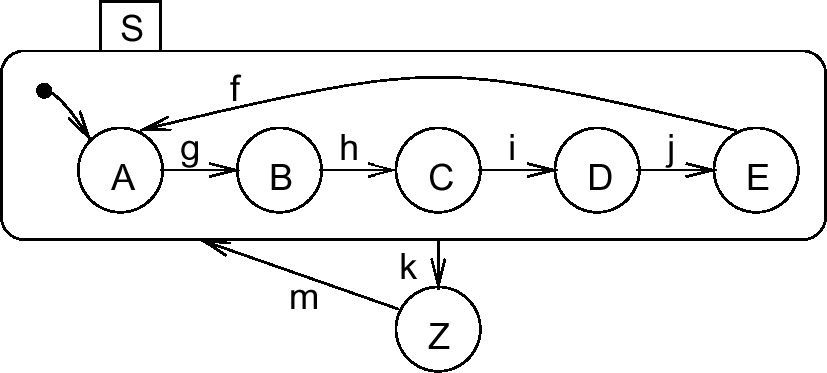
\includegraphics[width=\columnwidth]{images/statechart_default_state.png}
\end{minipage}


\subsection{History}

\begin{outline}
    \1 Wenn Input $m$ auftritt, wird in $S$ derjenige sub-state betreten, in welchem man war, \textbf{bevor $\bm{S}$ verlassen wurde}
        \2 Wenn $S$ zum ersten Mal betreten wird, ist der \textbf{default-Mechanismus} aktiv
    \1 History und Default-Mechanismus können hierarchisch verwendet werden
\end{outline}


\subsubsection{Shallow History}

\begin{itemize}
    \item Der Histroy-Mechanismus merkt sich den entsprechenden sub-state
    \item Kennzeichnung: $H$
\end{itemize}


\example{Shallow-History}

\begin{minipage}[c]{0.48\columnwidth}
    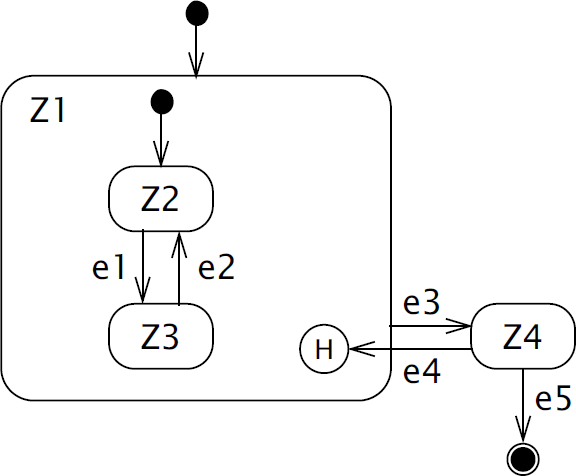
\includegraphics[width=\columnwidth]{images/statechart_shallow_history.png}
\end{minipage}
\hfill
\begin{minipage}[c]{0.48\columnwidth}
    \begin{itemize}
        \item In Zustand $Z3$ bewirkt der Event $e3$ einen Übergang zu $Z4$
        \item Der Event $e4$ führt nu zu einem Übergang zum früheren Zustand $Z3$
    \end{itemize}
\end{minipage}


\subsubsection{Deep History}

\begin{itemize}
    \item Der Histroy-Mechanismus merkt sich frühere Zustände \textbf{bis in die unterste Hierarchie}
    \item Kennezeichnung: $H^*$
\end{itemize}


\example{Deep-History}

\begin{minipage}[c]{0.48\columnwidth}
    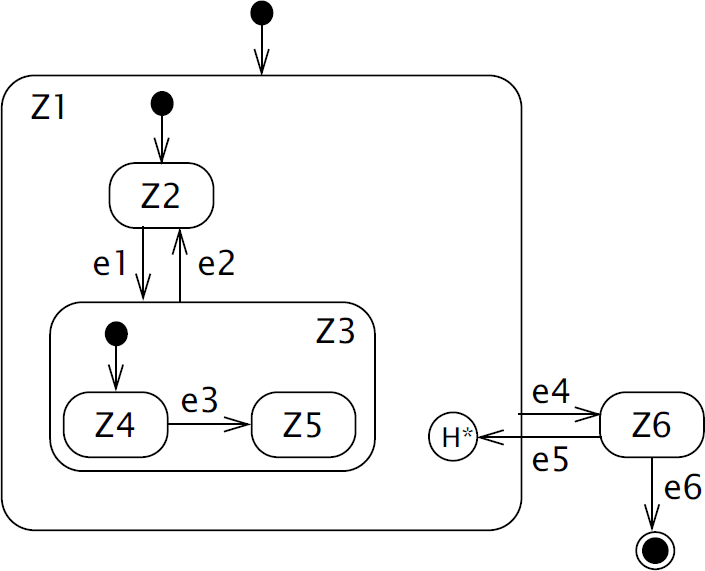
\includegraphics[width=\columnwidth]{images/statechart_deep_history.png}
\end{minipage}
\hfill
\begin{minipage}[c]{0.48\columnwidth}
    \begin{outline}
        \1 Im Zustand $Z5$ bewirkt der Event $e4$ einen Übergang zu $Z6$
        \1 Der Event $e5$ führt nun zu einem Übergang zum früheren Zustand $Z5$
            \2 Eine Shallow History würde bei $e5$ nur in den Zustand $Z3$, und damit in $Z4$, wechseln
    \end{outline}
\end{minipage}


\subsection{Kombination: History- und Default-Mechanismus}

Folgende statecharts bilden genau das Gleiche ab

\vspace{0.2cm}

\begin{minipage}[c]{0.41\columnwidth}
    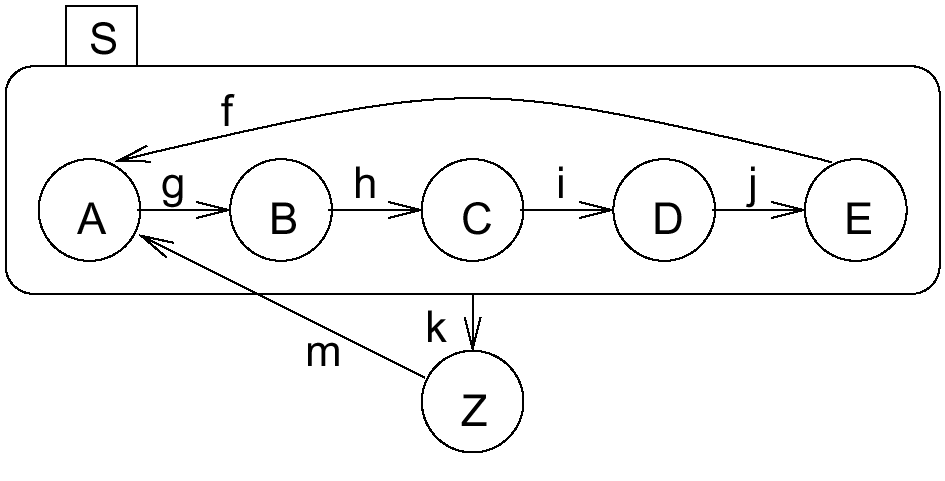
\includegraphics[width=\columnwidth]{images/statechart_hierarchie.png}
\end{minipage}
\hfill
\begin{minipage}[c]{0.07\columnwidth}
    \begin{center}
        \huge \textlrarrow\
    \end{center}
\end{minipage}
\hfill
\begin{minipage}[c]{0.41\columnwidth}
    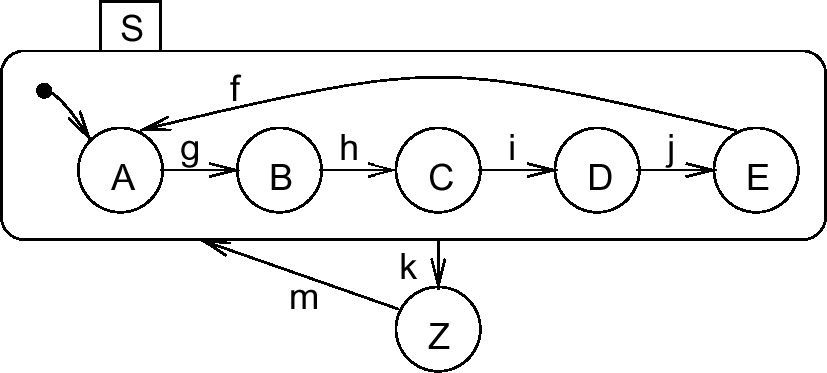
\includegraphics[width=\columnwidth]{images/statechart_default_state.png}
\end{minipage}


\subsection{Parallelität (AND-super-state, Teilautomaten)}

\begin{itemize}
    \item Die FSM befindet sich in \textbf{allen} sub-states von einem super-state $S$, wenn $S$ aktiv ist.\\
        (\textrightarrow\ in $A$ \textbf{AND} in $B$ \textbf{AND} ...)
\end{itemize}

\begin{center}
    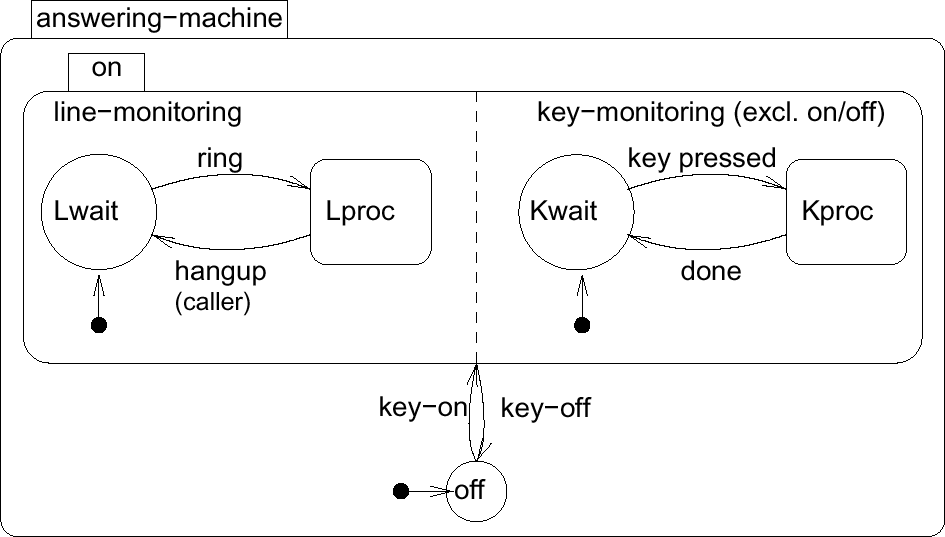
\includegraphics[width=0.75\columnwidth]{images/statechart_concurrency.png}
\end{center}


\subsection{Timers}

\begin{itemize}
    \item Wenn Evend $a$ nicht eintritt, während das System für $20 \, \milli \second$ im linken state ist, wird ein timeout passieren
    \item Eigentlich sind Timers nicht nötig, da die Wartezeit auch als Übergangsbedingung (Ereignis) zwischen zwei states formuliert werden könnte
\end{itemize}

\begin{center}
    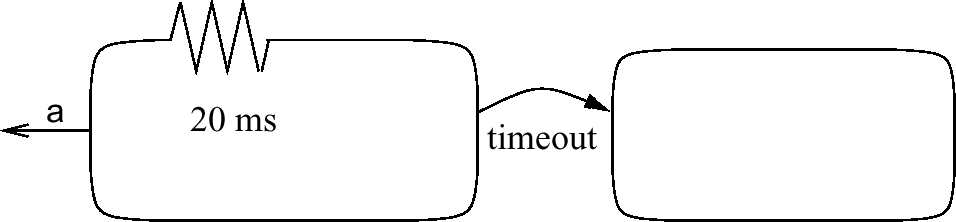
\includegraphics[width=0.65\columnwidth]{images/statechart_timers.png}
\end{center}


\subsection{Beispiel -- Armbanduhr als Statechart}  %CHECK: vielleicht gibt es im Praktikum ein besseres Beispiel...?

\begin{center}
    % 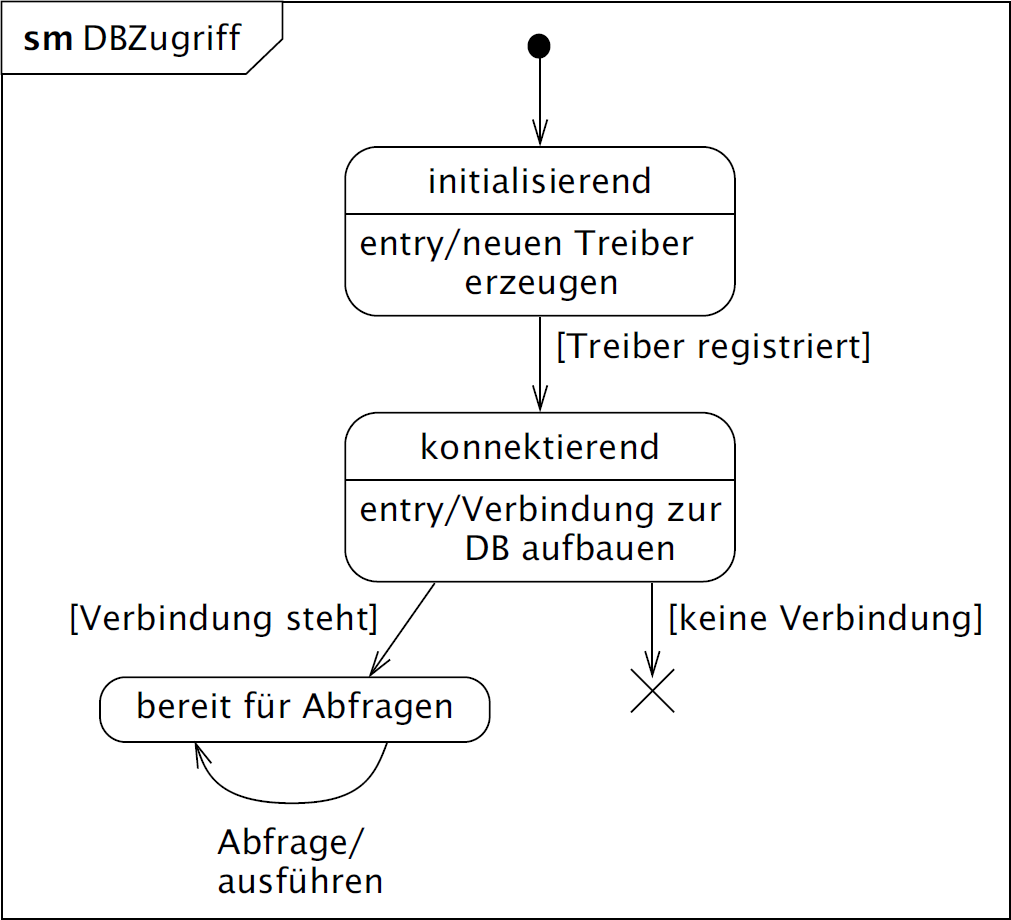
\includegraphics[width=0.8\columnwidth]{images/statechart_example.png}
    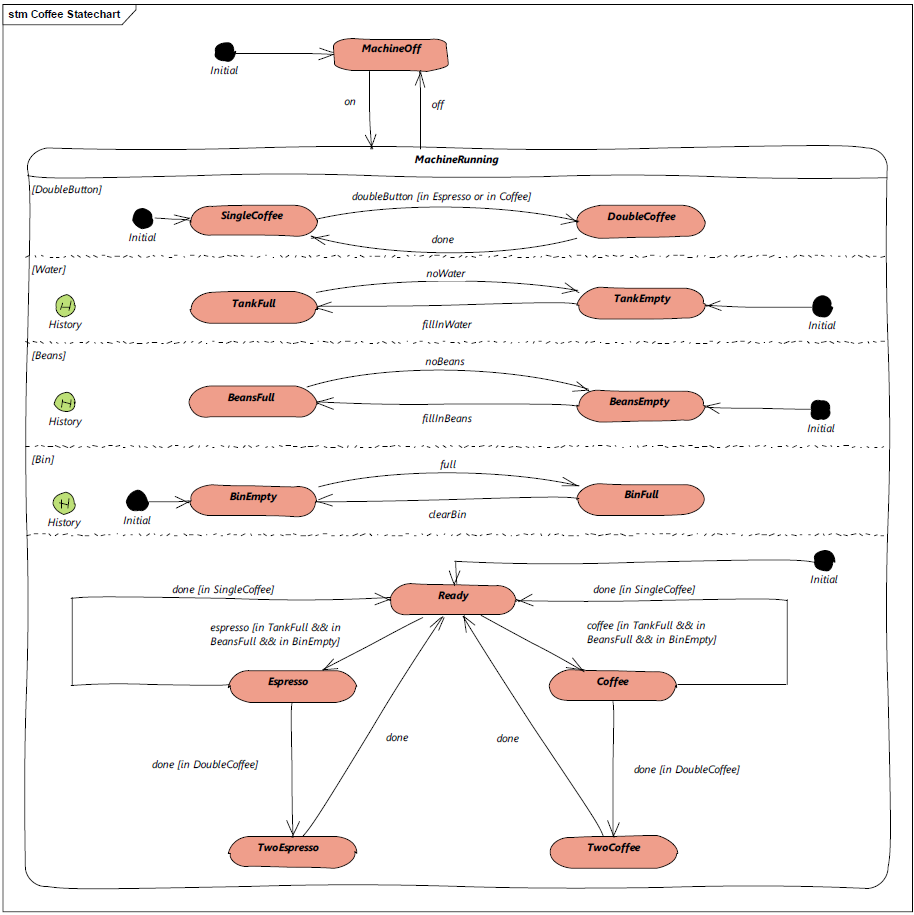
\includegraphics[width=0.8\columnwidth]{images/statechart_example_coffeemachine.png}    %TODO: insert as pdf
\end{center}

